\documentclass[10pt,a4paper,landscape]{article}
% -- Layout ----
\usepackage[top=0.6cm, bottom=0.6cm, left=0.5cm, right=0.5cm, landscape]{geometry}

% -- Titles ----
\usepackage[
  tiny,                     % text size title
  compact                   % reduce vertical space before/after title
]{titlesec}
% \titlespacing*
\titleformat{\section}{\normalfont\small\bfseries}{\thesection}{0em}{} % Remove space before and after section titles
\titleformat{\subsection}{\normalfont\small\bfseries}{\thesubsection}{0em}{} % Remove space before and after subsection titles
\titlespacing*{\section}{0pt}{0pt}{0pt} % Remove space before/after section titles
\titlespacing*{\subsection}{0pt}{0pt}{0pt} % Remove space before/after subsec titles

% -- Colors ----
\usepackage[dvipsnames]{xcolor}
\definecolor{dmm}{RGB}{192,192,192} % Define a custom dimmed text color
\definecolor{cmt}{RGB}{61,123,123}

% -- Math ------
\usepackage{mathtools}
\usepackage{amssymb}
\usepackage{turnstile}%better vdash

% -- Lists -----
\usepackage[inline]{enumitem}
\setlist{noitemsep}% Remove vspace between items
% Set vspace before and after  list environments as well as the left margin
\setlist[itemize,1]{leftmargin=.6em,labelindent=0pt,labelsep=2pt,
  topsep=1pt,partopsep=1pt}
\setlist[enumerate,1]{leftmargin=1em,labelindent=0pt,labelsep=2pt,
  topsep=1pt,partopsep=1pt}
\setlist[itemize,2]{leftmargin=.3em,labelindent=1pt,topsep=1pt,partopsep=1pt}
\setlist[enumerate,2]{leftmargin=0.2em,labelindent=1pt,topsep=1pt,partopsep=1pt}
\setlist[description]{labelwidth=\linewidth,font=\small\bfseries,leftmargin=1em,topsep=1pt,partopsep=1pt}
% -- Code listing ---
\usepackage{listings}
\lstset{
  aboveskip=3pt,
  belowskip=3pt,
  basicstyle=\small\ttfamily,
  breaklines=true,
  % commentstyle=\upshape\ttfamily,
  captionpos=b,
  commentstyle=\color{cmt},
  columns=flexible,
  frame=single,
  keepspaces=false,
  keywordstyle=\bfseries,
  showspaces=false,
  showstringspaces=false,
  showtabs=false,
  tabsize=2,
}

% Parse Trees
\usepackage{tikz}
\usetikzlibrary{ arrows, automata, bbox, calc, positioning, tikzmark, decorations.pathmorphing, decorations.pathreplacing, decorations.shapes, }
\tikzset{
  >=stealth',
  node distance=1cm,
  recstate/.style={
    circle,draw=blue!50,fill=blue!20,thick,font=\small\sffamily,rounded corners=3pt,
    minimum size=1cm,inner sep=1pt
  },
  ivp/.style={draw,->,auto,font=\small\sffamily,bend angle=60},
  msi/.style={draw=Brown,->,auto,font=\small\sffamily,bend angle=80},
  msibs/.style={draw=RoyalBlue,->,auto,font=\small\sffamily,bend angle=80},
  msinl/.style={font=\footnotesize\sffamily}, %msi node label
  every edge/.style={draw,auto,font=\small\sffamily},
  every loop/.style={looseness=4},
  initial text=start,initial where=right
}

% Place a figure env right here via [H] option
\usepackage{float}

% Side by side figure
\usepackage{subcaption}
% \usepackage{caption}
% \captionsetup{belowskip=0pt, aboveskip=0pt}
\usepackage{pifont}

% -- Multi-Col layout --
\usepackage{multicol}

% No indentation
\setlength\parindent{0pt}
\setlength\abovedisplayskip{-5pt}
\setlength\belowdisplayskip{-5pt}
\setlength\abovedisplayshortskip{-4pt}
\setlength\belowdisplayshortskip{-4pt}
\setlength\tabcolsep{5pt}
\newcommand{\gor}{\;|\;}
\newcommand{\num}{\texttt{\#}~}
\newcommand{\pro}[1]{\textcolor{Brown}{#1}}
\newcommand{\bus}[1]{\textcolor{RoyalBlue}{#1}}
\renewcommand{\arraystretch}{1.2}


\begin{document}
% Suppress page number for all pages
\pagestyle{empty}
% Each section goes into this env
\begin{multicols*}{3}
% \section*{LR(0) item, closure, goto}
\begin{itemize}
\item \mb{item}: a grammar rule with a dot(\textbf{.}) that indicates a
  parser position in its RHS: $A \to \alpha\beta\gamma$ generates 4 LR(0) items:
  \begin{align*}
    A &\to \lrd\alpha\beta\gamma \\
    A &\to \alpha\lrd\beta\gamma \\
    A &\to \alpha\beta\lrd\gamma \\
    A &\to \alpha\beta\gamma\lrd
  \end{align*}
\item $X \to\varepsilon$ has its own item: $X\to\lrd$
\item When dot already at the end, no change to the item $X\to A\lrd$
\item \mb{closure}: for item $A\to\alpha\lrd B\beta$ where $B$ is a \mo{non-terminal}. If $B$ has multiple productions $B\to \gamma_1 \gor \cdots \gor \gamma_n$, then \mo{all} $B\to\lrd\gamma_i\;(1 \leq i \leq n)$ should be in the same state as the item
\item \mb{goto}: for item $A\to\alpha\lrd X\beta$ where $X$ can be a terminal or non-terminal, then create a new state that must contains
  \begin{enumerate}
  \item item $A\to\alpha X\lrd\beta$ (i.e. pass $X$), plus
  \item the closure of the above item
  \end{enumerate}
\item \textbf{closure} is about adding new \textbf{items} to a LR(0) DFA state
\item \textbf{goto} is about creating transitions and states in LR(0) DFA
\end{itemize}
\section*{Example: create LR(0) DFA (parsing table and states)}
\begin{align*}
  S&\to (L)   \tag{1} \\
  S&\to x     \tag{2} \\
  L&\to S     \tag{3} \\
  L&\to L,S   \tag{4}
\end{align*}

\section*{Step 1: Augment the grammar to include a start symbol}
\begin{align*}
  S'&\to S\$  \tag{0} \\
  S&\to (L)   \tag{1} \\
  S&\to x     \tag{2} \\
  L&\to S     \tag{3} \\
  L&\to L,S   \tag{4}
\end{align*}
Also if there is any rule like $X\to N_1 \gor N_2 \dots$, rewrite it to
\begin{align*}
  X\to N_1 & X\to N_2 \cdots
\end{align*}
\section*{Step 2: Create start state for LR(0) DFA}
\begin{enumerate}
\item start with \textbf{starting item} $S'\to \lrd S\$$ and create state 1
  \begin{center}
    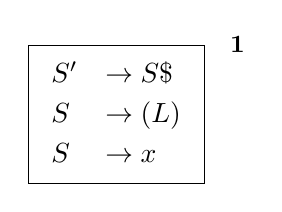
\begin{tikzpicture}[state/.style=draw]
    \node (s1) [state] {
      \begin{tabular}{ll}
         $S'$ & $\to\lrd S\$$  \\
         $S$  & $\to\lrd (L)$  \\
         $S$  & $\to\lrd x$
      \end{tabular}
    };
    \node (m1) [right=2mm of s1.north east,font=\bf\small]{1};
    \end{tikzpicture}
  \end{center}
\item there is no non-terminals before \mr{\textbf{.}} so need \textbf{goto}
\item In state 1, use goto to create edges and new states
  \begin{itemize}
  \item \textbf{goto}($x$) $\Rightarrow$ state 2
  \end{itemize}
  \begin{center}
    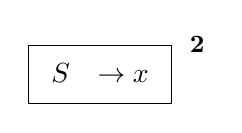
\begin{tikzpicture}[state/.style=draw]
      \node (s2) [state] {
        \begin{tabular}{ll}
          $S$ & $\to x\lrd$
        \end{tabular}
      };
      \node (m2) [right=1mm of s2.north east,font=\bf\small]{2};
    \end{tikzpicture}
  \end{center}
  \begin{itemize}
  \item \textbf{goto}(left-paren) $\Rightarrow$ state 3
  \end{itemize}
  \begin{center}
    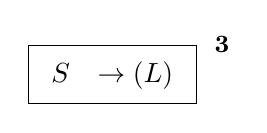
\begin{tikzpicture}[state/.style=draw]
      \node (s3) [state] {
        \begin{tabular}{ll}
          $S$ & $\to (\lrd L)$
        \end{tabular}
      };
      \node (m3) [right=1mm of s3.north east,font=\bf\small]{3};
    \end{tikzpicture}
  \end{center}
\item In state 3, $L$ is a non-terminal so need to add \textbf{closure}($L$)
\item[] Similarly, $S$ is a non-termina so need to add \textbf{closure}($S$) when done with $L$. Last two items also appear in state 1
  \begin{center}
    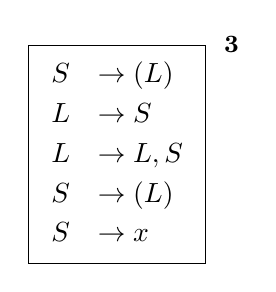
\begin{tikzpicture}[state/.style=draw]
    \node (s3) [state] {
      \begin{tabular}{ll}
         $S$ & $\to (\lrd L)$ \\
         $L$ & $\to \lrd S$ \\
         $L$ & $\to \lrd L,S$ \\
         $S$ & $\to \lrd (L)$ \\
         $S$ & $\to \lrd x$ \\
      \end{tabular}
    };
    \node (m3) [right=1mm of s3.north east,font=\bf\small]{3};
    \end{tikzpicture}
  \end{center}
\item In state 1, \textbf{goto}($S$) and get state 4
  \begin{center}
    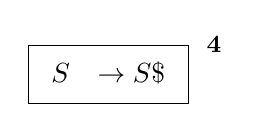
\begin{tikzpicture}[state/.style=draw]
    \node (s4) [state] {
      \begin{tabular}{ll}
         $S$ & $\to S\lrd\$$
      \end{tabular}
    };
    \node (m4) [right=1mm of s4.north east,font=\bf\small]{4};
    \end{tikzpicture}
  \end{center}
\item In state 3, closure is done, we need goto (start with easy)
  \begin{itemize}
  \item \textbf{goto}($x$), item $S\to x\lrd \Rightarrow$ existing state 2
  \item \textbf{goto}(\textsf{left-pare}), item $S\to (\lrd L)\Rightarrow$ existing state 3
  \item \textbf{goto}($L$), item $S\to (L\lrd)\Rightarrow$ new state 5
  \item \textbf{goto}($L$), item $L\to L\lrd,S\Rightarrow$ new state 5
  \begin{center}
    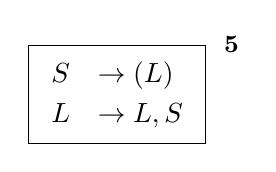
\begin{tikzpicture}[state/.style=draw]
    \node (s5) [state] {
      \begin{tabular}{ll}
         $S$ & $\to (L\lrd)$ \\
         $L$ & $\to L\lrd,S$
      \end{tabular}
    };
    \node (m5) [right=1mm of s5.north east,font=\bf\small]{5};
    \end{tikzpicture}
  \end{center}
  \item \textbf{goto}($S$), item $L\to S\lrd\Rightarrow$ new state 7
  \begin{center}
    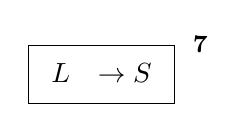
\begin{tikzpicture}[state/.style=draw]
    \node (s7) [state] {
      \begin{tabular}{ll}
         $L$ & $\to S\lrd$
      \end{tabular}
    };
    \node (m7) [right=1mm of s7.north east,font=\bf\small]{7};
    \end{tikzpicture}
  \end{center}
  \end{itemize}
\item In state 5, need \textbf{goto} as there's no closure to be computed
  \begin{itemize}
  \item \textbf{goto}(\textsf{right-paren}), item $S\to (L)\lrd \Rightarrow$ new state 6
    \begin{center}
      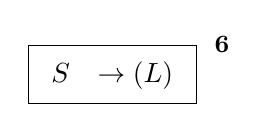
\begin{tikzpicture}[state/.style=draw]
        \node (s6) [state] {
          \begin{tabular}{ll}
            $S$ & $\to (L)\lrd$
          \end{tabular}
        };
        \node (m6) [right=1mm of s6.north east,font=\bf\small]{6};
      \end{tikzpicture}
    \end{center}
  \item \textbf{goto}(,), item $L\to L,\lrd S \Rightarrow$ new state 8
    \begin{center}
      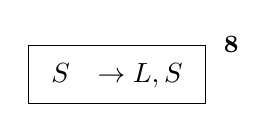
\begin{tikzpicture}[state/.style=draw]
        \node (s8) [state] {
          \begin{tabular}{ll}
            $S$ & $\to L,\lrd S$
          \end{tabular}
        };
        \node (m8) [right=1mm of s8.north east,font=\bf\small]{8};
      \end{tikzpicture}
    \end{center}
  \end{itemize}
\item In state 8, $S$ is non-terminal so need add \textbf{closure}($S$)
  \begin{center}
    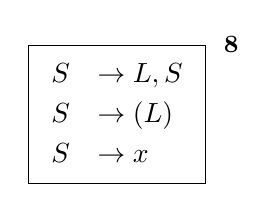
\begin{tikzpicture}[state/.style=draw]
      \node (s8) [state] {
        \begin{tabular}{ll}
          $S$ & $\to L,\lrd S$ \\
          $S$ & $\to \lrd(L)$ \\
          $S$ & $\to \lrd x$
        \end{tabular}
      };
      \node (m8) [right=1mm of s8.north east,font=\bf\small]{8};
    \end{tikzpicture}
  \end{center}
\item In state 8, now apply goto rule:
  \begin{itemize}
  \item \textbf{goto}($S$), item $S\to (L,S)\lrd \Rightarrow$ new state 9
    \begin{center}
      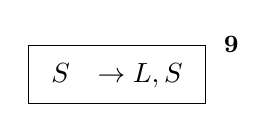
\begin{tikzpicture}[state/.style=draw]
        \node (s9) [state] {
          \begin{tabular}{ll}
            $S$ & $\to L,S\lrd$ \\
          \end{tabular}
          % $S\to (L,S)\lrd$
        };
        \node (m9) [right=1mm of s9.north east,font=\bf\small]{9};
      \end{tikzpicture}
    \end{center}
  \item \textbf{goto}(\textsf{left-paren}), item $S\to (\lrd L) \Rightarrow$ existing state 3
  \item \textbf{goto}($x$), item $S\to x\lrd \Rightarrow$ existing state 2
  \end{itemize}
\end{enumerate}
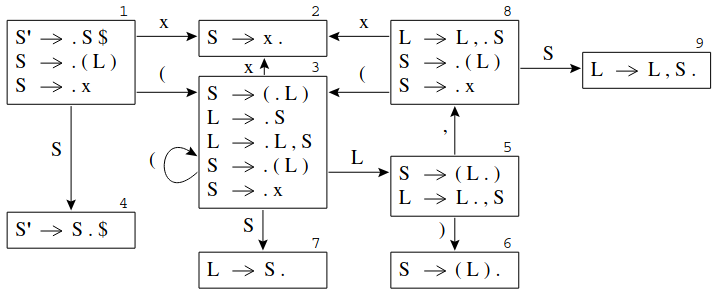
\includegraphics[width=\linewidth]{img/LR0}
\section*{Step 3: draw parse table (row is state, col is symbol)}

\begin{itemize}
\item In edege $I\overset{X}{\to} J$, if $X$ is \mb{terminal}, \emph{shift} $J$ at $(I,X)$
\item In edege $I\overset{X}{\to} J$, if $X$ is \mb{non-terminal}, \emph{goto} $J$ at $(I,X)$
\item For each $I$ with an item $S'\to S\lrd\$$, \mb{accept} at $(I,\$)$
\item For any $I$ with item $A\to \gamma\lrd$, \mb{reduce $n$} ($n$ is this production's num in the grammar) at $(I,Y)$ for every $Y$
\end{itemize}
\begin{tabular}{r|lllll|ll}
  state $I$& (   & )   & $x$ &,    & $\$$ & $S$  & $L$ \\
  \hline
  1        &$s3$ &     &$s2$ &     &      & $g4$ &      \\
  2        &$r2$ &$r2$ &$r2$ &$r2$ & $r2$ &      &      \\
  3        &$r3$ &     &$r2$ &     &      & $g7$ & $g5$ \\
  4        &     &     &     &     & $a$  &      &    \\
  5        &     &$s6$ &     &$s8$ &      &      &    \\
  6        &$r1$ &$r1$ &$r1$ &$r1$ &$r1$  &      &    \\
  7        &$r3$ &$r3$ &$r3$ &$r3$ &$r3$  &      &    \\
  8        &$s3$ &     &$s2$ &     &      & $g9$ &    \\
  9        &$r4$ &$r4$ &$r4$ &$r4$ &$r4$  &      &    \\
  \hline
\end{tabular}

% \section*{Conflicts in LR parsing}
\begin{itemize}
\item \mb{shift} the dot past the input symbol currently before the dot
\item[] Before: $X\to \lrd A\beta$; After: $X\to A\lrd\beta$
\item \mb{reduce}: when dot at the end of item, RHS of the production can be replaced with the LHS
\item In a state $I$, expect to have either a reduce or a shift action, not both. Otherwise, there is a \mo{conflict}:
  \begin{enumerate}
  \item \mb{S}/\mb{R} conflict: state $I$ has a reduce \textbf{AND} a shift action
  \item \mb{R}/\mb{R} conflict: state $I$ has two reduce actions
  \end{enumerate}
\end{itemize}
\section*{Example: A grammar with S/R conflict}
\begin{minipage}{.5\linewidth}
\begin{align*}
  _0\quad S&\to E\$   \\
  _1\quad E&\to T + E
\end{align*}
\end{minipage}
\begin{minipage}{.5\linewidth}
\begin{align*}
  _2\quad E&\to T \\
  _3\quad T&\to x
\end{align*}
\end{minipage}
\section*{grammar DFA with R/S conflict}
\begin{tikzpicture}
  % I1
  \node (i1) [lrst, anchor=north east] {
    $S\to \lrd E\$$\\
    $E\to \lrd T + E$\\
    $E\to \lrd T$\\
    $T\to \lrd x$
  };
  \node [above=1mm of i1.north east, font=\footnotesize\bf]{1};

  %I2
  \node (i2) [lrst, right=12mm of i1.north east, anchor=north west] {
    $S\to E\lrd\$$
  };
  \node (m2) [above=1mm of i2.north east, font=\footnotesize\bf]{2};

  %I3
  \node (i3) [lrst, right=12mm of i1.east, anchor=north west] {
    $E\to T\lrd + E$\\
    $E\to T\lrd $
  };
  \node (m3) [right=1mm of i3.north east, font=\footnotesize\bf]{3};

  %I5
  \node (i5) [lrst, below=15mm of i1.south, anchor=north] {
    $T\to x\lrd$
  };
  \node (m5) [above=1mm of i5.north east, font=\footnotesize\bf]{5};

  %I4
  \node (i4) [lrst, below=6mm of i3, anchor=north] {
    $E\to T + \lrd E$\\
    $E\to \lrd T$\\
    $E\to \lrd T + E$ \\
    $T\to \lrd x$
  };
  \node (m4) [right=1mm of i4.north east, font=\footnotesize\bf]{4};

  %I6
  \node (i6) [lrst, right=10mm of i4, anchor=west] {
    $E\to T + E\lrd$
  };
  \node (m6) [above=1mm of i6.north east, font=\footnotesize\bf]{6};

  % note
  \node(note)[right=8mm of i3.north east, anchor=west, text width=3cm, font=\small] {
    In $I_3$, there are a shift action (over $+$) and a reduce action (dot at the end) $\to$ a S/R conflict in $I_3$ and the grammar is \mr{not} LR(0)
  };

  % paths
  \draw[->] (i1.east |- i2.west) -- (i2.west) node[midway, above]{$E$}  ;
  \draw[->] (i1.mid east |- i3.west) -- (i3.west) node[midway, above]{$T$}  ;
  \draw[->] (i1) edge node[left]{$x$} (i5) ;
  \draw[->]
  ([xshift=4mm]i3.south) -- ([xshift=4mm]i4.north) node[midway,right] {$+$};
  \draw[->]
  ([xshift=-4mm]i4.north) -- ([xshift=-4mm]i3.south) node[midway,left] {$T$};
  \draw[->] (i4) edge node[above]{$E$} (i6);
  \draw[->] (i4.west |- i5.east) -- (i5.east) node[midway, above]{$x$};

\end{tikzpicture}
\section*{Grammar parse table with R/S conflict}
\begin{minipage}{.7\linewidth}
\begin{center}
\begin{tabular}{l|lll|ll}
  State &\multicolumn{3}{c}{Action$^1$} & \multicolumn{2}{c}{Goto$^2$}  \\
  \hline
  $I$ & + & $x$  &\$       & $T$ & $E$  \\
  \hline
   1  &   & $s5$ &         &$g3$& $g2$ \\
   2  &   &      &$a$      && \\
   3  &$s4,r2$&$r2$&$r2$   && \\
   4  &   &$s5$&           &$g3$&$g6$ \\
   5  &$r3$&$r3$&$r3$      &    & \\
   6  &$r1$&$r1$&$r1$      &    & \\
  \hline
  \multicolumn{6}{l}{\footnotesize 1: Action (s/r) only on terminals and \$}\\
  \hline
  \multicolumn{6}{l}{\footnotesize 2: Goto only on non-terminals}\\
  \hline
\end{tabular}
\end{center}
\end{minipage}
\begin{minipage}{.3\linewidth}
  {\small
    In state 3, on symbol +, there is a duplicate entry: The parser must shift
    into state 4 and also reduce by production 2. This is a conflict and indicates
    that the grammar is \mr{not} LR(0).
  }
\end{minipage}
\section*{Use FOLLOW to build SLR and remove S/R conflict}
\begin{enumerate}
\item in each state $I$, identify all the reduce items like $A\to \alpha\lrd$ (dot at the end) where $\alpha \in \Sigma$ (terminals plus \$).
  \begin{itemize}
  \item In $I_2$, $S\to E\lrd\$$, need  $\mfn{follow}(S)$
  \item In $I_3$, $E\to T\lrd$, need $\mfn{follow}(E)$
  \item In $I_5$, $T\to x\lrd$, need $\mfn{follow}(T)$
  \item In $I_6$, $E\to T + E\lrd$, need $\mfn{follow}(E)$
  \end{itemize}
\item for each reduce item above, compute \textsf{FOLLOW}(LHS)
  \begin{itemize}
  \item $\mfn{follow}(S) = \mset{\$}$ (just init the set to include \$)
  \item $\mfn{follow}(T) = \mfn{follow}(E) \cup \mfn{first}(+) = \mset{+,\$}$
  \item $\mfn{follow}(E) = \mset{\$}$
  \end{itemize}
\item for each token $X$ in each computed follow set above, put a reduce action $(I, X, A\to \alpha)$ (on lookahead $X$, reduce by rule $A\to \alpha$) in SLR table
  \begin{itemize}
  \item $(I_2, \$, S\to E\$)$, put $a$ ($r0$) at $(I_2, \$)$
  \item $(I_3, \$, E\to T)$, put $r2$ at $(I_3, \$)$
  \item $(I_5, +, T\to x)$, put $r3$ at $(I_5, +)$
  \item $(I_5, \$, T\to x)$, put $r3$ at $(I_5, \$)$
  \item $(I_6, \$, E\to T + E)$, put $r1$ at $(I_6, \$)$
  \end{itemize}
\end{enumerate}
\begin{center}
\begin{tabular}{l|lll|ll}
  State &\multicolumn{3}{c}{Action} & \multicolumn{2}{c}{Goto}  \\
  \hline
  $I$ & + & $x$  &\$       & $T$ & $E$  \\
  \hline
   1  &   & $s5$ &         &$g3$& $g2$ \\
   2  &   &      &$a$      &    & \\
   3  &$s4$&     &$r2$     && \\
   4  &   &$s5$&           &$g3$&$g6$ \\
   5  &$r3$&&$r3$          &    & \\
   6  &    &    &$r1$      &    & \\
  \hline
\end{tabular}
\end{center}

\section*{LR(1) items $(A\to \alpha\lrd\beta, x)$ with 3 parts; closure, goto}
\begin{itemize}
\item a grammar production: $A\to\ldots$
\item a right-hand-side position (represent by the \mr{dot} $\lrd$)
\item a lookahead symbol $(A\to \alpha\lrd\beta, \mo{x})$
\item The idea is that an item $(A\to\alpha\beta\lrd,x)$ indicates that
  \begin{itemize}
  \item the sequence $\alpha$ is on top of the stack
  \item at the head of the input is a string derivable from $\beta x$
  \end{itemize}
\item $\beta$ can be terminal or non-terminal, $x$ can be $\$$(\texttt{EOF})
\item In pseudo code, $X$ in item $(A\to \alpha\lrd X\beta, z)$ is non-terminal
\end{itemize}
\includegraphics*[width=\linewidth]{img/LR1_closure_goto}
\section*{Example: A LR(1) grammar and its parsing table}
\begin{minipage}{.5\linewidth}
\begin{align*}
  _0\quad S'&\to S\$  \\
  _1\quad S&\to V = E \\
  _2\quad S&\to E
\end{align*}
\end{minipage}
\begin{minipage}{.5\linewidth}
\begin{align*}
  _3\quad  E&\to V   \\
  _4\quad  V&\to x   \\
  _5\quad  V&\to *E
\end{align*}
\end{minipage}
\begin{itemize}
\item According to the pseudo code, lookahead for prod 0 is $\mfn{first}(\$)$. ``()'' around items are dropped for simplicity

  \begin{minipage}{\linewidth}
    \centering
    \begin{tikzpicture}
      \node (i0)[lrst] {
        \dm{(} $S' \to\lrd S$,\quad\mr{?} \dm{)}
      };
      \node (m1)[right=0.2mm of i0.north east,font=\small\bf] {\dm{1}};

      \node (i1)[lrst, right=20mm of i0.east] {
        $S' \to\lrd S$,\$
      };
      \node (m1)[right=1mm of i1.north east,font=\small\bf] {1};
      \draw[->] (i0) -- (i1);
    \end{tikzpicture}
  \end{minipage}
\item $S$ is non terminal, need to compute closure($I_1$):
  \begin{enumerate}
  \item Add items via closure rule; for each item, lookahead is unknown(?) for now, except prod 0
  \item For $S\to V = E$, $w=\mfn{first}(=E\$)$, need to add items $(V\to \lrd x, =)$ and $(V\to \lrd * E, =)$ to $I_1$
  \item For $S\to E$, $w=\mfn{first}(\$)$, $(E\to \lrd V, \$)$ already in $I_1$
  \item For $E\to V$, $w=\mfn{first}(\$) = \mset{\$}$, $(V\to \lrd\cdots, \$)$ in $I_1$
  \end{enumerate}
\end{itemize}
\begin{minipage}{\linewidth}
  \begin{tikzpicture}
    \node (i0)[lrst] {
      \begin{tabular}{ll}
        \dm{(} $S' \to\lrd S$   &, \$     \dm{)} \\
        \dm{(} $S \to\lrd V=E $ &, \mr{?} \dm{)} \\
        \dm{(} $S \to\lrd E   $ &, \mr{?} \dm{)} \\
        \dm{(} $E \to\lrd V   $ &, \mr{?} \dm{)} \\
        \dm{(} $V \to\lrd x   $ &, \mr{?} \dm{)} \\
        \dm{(} $V \to\lrd *E  $ &, \mr{?} \dm{)}
      \end{tabular}
    };
    \node (m0)[right=0.2mm of i0.north east,font=\small\bf] {\dm{1}};

    \node (i1)[lrst, right=6mm of i0.east] {
      \begin{tabular}{ll}
        $S' \to\lrd S$   &, \$ \\
        $S \to\lrd V=E $ &, \$  \\
        $S \to\lrd E   $ &, \$ \\
        $E \to\lrd V   $ &, \$ \\
        $V \to\lrd x   $ &, \$ $\gor$ = \\
        $V \to\lrd *E  $ &, \$ $\gor$ =
      \end{tabular}
    };
    \node (m1)[right=0.1mm of i1.north east,font=\small\bf] {1};
    \draw[->] (i0) -- (i1);
  \end{tikzpicture}
\end{minipage}
\begin{itemize}
\item Repeat the above steps to get the entire DFA diagram
\end{itemize}
\includegraphics*[width=\linewidth]{img/LR1_DFA}
\includegraphics*[width=\linewidth]{img/LR1_parsing_table}
\begin{itemize}
\item Wherever dot at a prod end, there is a reduce for that prod
\item Whenever dot is to the left of a terminal or non-terminal, there is a corresponding shift or goto
\end{itemize}

% \section*{Example of LR(1) DFA and parsing table $a.k.a$ CLR(1)}
% \begin{minipage}{.5\linewidth}
\begin{align*}
  _1\quad S&\to XX \\
  _2\quad X&\to aX \\
  _3\quad X&\to b
\end{align*}
% \end{minipage}
% \begin{minipage}{.5\linewidth}
% \begin{align*}
%   _0\quad S'&\to S \\
%   _1\quad S&\to XX \\
%   _2\quad X&\to aX \\
%   _3\quad X&\to b
% \end{align*}
% \end{minipage}
\section*{Step 1: Add a new a start symbol (see above right)}
\begin{align*}
  _0\quad S'&\to S \\
  _1\quad S&\to XX \\
  _2\quad X&\to aX \\
  _3\quad X&\to b
\end{align*}
\section*{Step 2: Compute closures and gotos to build the DFA}
\begin{itemize}
\item For start state $I_0$, compute \textbf{closure}($I_0$) and \textbf{goto}($I_0$). For special prod $S'\to S\$$, its lookahead is \textbf{always} \$
\begin{minipage}{\linewidth}
  \centering
  \begin{tikzpicture}
    \node (i0) [lrst] {
      \begin{tabular}{ll}
        $S'\to \lrd S$ & ,\$
      \end{tabular}
    };
    \node (m0) [right=0.1mm of i0.north east,font=\footnotesize\bf] {0};
  \end{tikzpicture}
\end{minipage}
\item $S$ is non-terminal, need to add new items to $I_0$


\end{itemize}
\begin{minipage}{\linewidth}
  \begin{tikzpicture}
    \node (i0) [lrst] {
      \begin{tabular}{ll}
        $S'\to \lrd S$ & ,\$ \\
        $S\to \lrd XX$ & ,\mr{?}
      \end{tabular}
    };

    \node (i1) [lrst,right=2mm of i0.east] {
      \begin{tabular}{ll}
        $S'\to \lrd S$ & ,\$ \\
        $S\to \lrd XX$ & ,$\mfn{first}(\$)$
      \end{tabular}
    };

    \node (i2) [lrst,right=2mm of i1.east] {
      \begin{tabular}{ll}
        $S'\to \lrd S$ & ,\$ \\
        $S\to \lrd XX$ & ,\$
      \end{tabular}
    };
  \end{tikzpicture}
\end{minipage}
\begin{itemize}
\item $X$ is non-terminal, need to add new items
\end{itemize}
\begin{minipage}{\linewidth}
  \centering
  \begin{tikzpicture}
    \node (i1) [lrst,right=5mm of i0.east] {
      \begin{tabular}{ll}
        $S'\to \lrd S$ & ,\$ \\
        $S\to \lrd XX$ & ,$\mfn{first}(\$)$ \\
        $X\to \lrd aX$ & ,$\mfn{first}(X\$)$ \\
        $X\to \lrd b$ & ,$\mfn{first}(X\$)$
      \end{tabular}
    };
    \node (m1) [right=0.1mm of i1.north east,font=\footnotesize\bf] {\dm{0}};

    \node (i2) [lrst,right=5mm of i1.east] {
      \begin{tabular}{ll}
        $S'\to \lrd S$ & ,\$ \\
        $S\to \lrd XX$ & ,\$ \\
        $X\to \lrd aX$ & ,$a \gor b$ \\
        $X\to \lrd b$  & ,$a \gor b$
      \end{tabular}
    };
    \node (m2) [right=0.1mm of i2.north east,font=\footnotesize\bf] {0};

    \draw[->] (i1) -- (i2);
  \end{tikzpicture}
\end{minipage}
\begin{itemize}
\item when $I$ \textbf{goto} $I'$, item$_1$ in $I'$ copies LA from its prev in $I$
\end{itemize}
\begin{minipage}{\linewidth}
  \begin{tikzpicture}
    % I0
    \node (i0) [lrst] {
      \begin{tabular}{ll}
        $S'\to \lrd S$ & ,\$ \\
        $S\to \lrd XX$ & ,\$ \\
        $X\to \lrd aX$ & ,$a \gor b$ \\
        $X\to \lrd b$  & ,$a \gor b$
      \end{tabular}
    };
    \node (m0) [above=0.1mm of i0.north east,font=\footnotesize\bf] {0};

    %I1
    \node (i1) [lrst,right=10mm of i0.north east, anchor=north west] {
      \begin{tabular}{ll}
        $S'\to S\lrd$ & ,\$ \\
      \end{tabular}
    };
    \node (m1) [above=0.1mm of i1.north east,font=\footnotesize\bf] {1};

    %I2
    \node (i2) [lrst,below=3mm of i1] {
      \begin{tabular}{ll}
        $S\to X\lrd X$ & ,\$ \\
        $X \to \lrd aX$ & ,\$ \\
        $X \to \lrd b$  & ,\$
      \end{tabular}
    };
    \node (m2) [above=0.1mm of i2.north east,font=\footnotesize\bf] {2};
    \node (note2) [right=1.5mm of i2.east,text width=2.5cm, font=\footnotesize]{
      In new state $I_2$, item$_1$ copies over \mo{LA}s from its prev in $I_0$:
      $S\to X\lrd X$ in $I_2$ copies \mo{\$} from $S\to \lrd XX$ in $I_0$\\
    };

    %I3
    \node (i3) [lrst,below=8mm of i0.south west, anchor=north west] {
      \begin{tabular}{ll}
        $X \to b\lrd$  & ,$a \gor b$
      \end{tabular}
    };
    \node (m3) [above=0.1mm of i3.north west,font=\footnotesize\bf] {3};

    %I4
    \node (i4) [lrst,below left=8mm of i2.south,anchor=north] {
      \begin{tabular}{ll}
        $X \to a\lrd X$  & ,$a \gor b$ \\
        $X \to \lrd aX$  & ,$a \gor b$ \\
        $X \to \lrd b$  & ,$a \gor b$
      \end{tabular}
    };
    \node (m4) [above=0.1mm of i4.north east,font=\footnotesize\bf] {4};

    \node(note0)[below=2mm of i3, text width=3.2cm,font=\footnotesize] {
      In $I_4$, LAs of item$_2$ and item$_3$ are computed as $\mfn{first}(X\$) = a\gor b$
    };

    \draw[->] (i0.south -| i3.north) -- (i3.north) node[midway,left]{$b$};
    \draw[->] (i0.south) -- (i4.north) node[midway,right]{$a$};
    \draw[->] (i0.east) -- (i2.west) node[midway,above]{$X$};
    \draw[->] (i0.east |- i1.west) -- (i1.west) node[midway,above]{$S$};
  \end{tikzpicture}
\end{minipage}
\begin{itemize}
\item \textbf{goto}($I_2, a$) does \mr{\emph{not}} lead to $I_4$,  but lead to $I_6$
\end{itemize}
\begin{tikzpicture}
  % I2
  \node (i2) [lrst] {
    \begin{tabular}{ll}
      $S\to X\lrd X$ & ,\$ \\
      $X \to \lrd aX$ & ,\$ \\
      $X \to \lrd b$  & ,\$
    \end{tabular}
  };
  \node (m2) [above=0.1mm of i2.north east,font=\footnotesize\bf] {2};

  % I5
  \node (i5) [lrst,right=8mm of i2.north east,anchor=north west] {
    \begin{tabular}{ll}
      $S \to XX\lrd$  & ,\$
    \end{tabular}
  };
  \node (m5) [above=0.1mm of i5.north east,font=\footnotesize\bf] {5};

  % I6
  \node (i6) [lrst,below=5mm of i5] {
    \begin{tabular}{ll}
      $X \to a\lrd X$  & ,\$ \\
      $X \to \lrd aX$  & ,\$ \\
      $S \to \lrd b$   & ,\$ \\
    \end{tabular}
  };
  \node (m6) [above=0.1mm of i6.north east,font=\footnotesize\bf] {6};
  \node (note6)[
  right=4mm of m5.north east,anchor=north west,text width=2.8cm,font=\footnotesize] {
    In $I_2$, shift $a$ leads to $X\to a\lrd X,\$$, due to LA \$ (\mr{not} $a\gor b$), need a new state $I_6$ with all below items\\
    $(X\to \cdots, \mfn{first}(\$))$ added to $I_6$
  };

  % I7
  \node (i7) [lrst,below=5mm of i2] {
    \begin{tabular}{ll}
      $X \to \lrd b$  & ,\$
    \end{tabular}
  };
  \node (m7) [below=0.1mm of i7.south east,font=\footnotesize\bf] {7};

  % I8
  \node (i8) [lrst,right=6mm of i6.south east,anchor=south west] {
    \begin{tabular}{ll}
      $X \to aX\lrd $  & ,\$
    \end{tabular}
  };
  \node (m8) [below=0.1mm of i8.south east,font=\footnotesize\bf] {8};
  \draw[->] (i2.east |- i5.west) -- (i5.west) node[midway, above]{$X$};
  \draw[->] (i2.east) -- (i6.west) node[midway, above]{$a$};
  \draw[->] (i2.south) -- (i7.north) node[midway, left]{$b$};
  \draw[->] (i6.west |- i7.east) -- (i7.east) node[midway, above]{$b$};
  \draw[->] (i6.east |- i8.west) -- (i8.west) node[midway, above]{$X$};
  \draw[->]
  ([xshift=4mm]i6.south west) to [bend right=60] node[above]{$a$}
  ([xshift=-4mm]i6.south east);
\end{tikzpicture}
\begin{itemize}
\item \mb{complete DFA} is therefore constructed as
\end{itemize}
\begin{minipage}{\linewidth}
  \begin{tikzpicture}
    % I0
    \node (i0) [lrst] {
      \begin{tabular}{ll}
        $S'\to \lrd S$ & ,\$ \\
        $S\to \lrd XX$ & ,\$ \\
        $X\to \lrd aX$ & ,$a \gor b$ \\
        $X\to \lrd b$  & ,$a \gor b$
      \end{tabular}
    };
    \node (m0) [above=0.1mm of i0.north east,font=\footnotesize\bf] {0};

    % I1
    \node (i1) [lrst,right=10mm of i0.north east, anchor=north west] {
      \begin{tabular}{ll}
        $S'\to S\lrd$ & ,\$ \\
      \end{tabular}
    };
    \node (m1) [above=0.1mm of i1.north east,font=\footnotesize\bf] {1};

    % I2
    \node (i2) [lrst,below=3mm of i1] {
      \begin{tabular}{ll}
        $S\to X\lrd X$ & ,\$ \\
        $X \to \lrd aX$ & ,\$ \\
        $X \to \lrd b$  & ,\$
      \end{tabular}
    };
    \node (m2) [above=0.1mm of i2.north east,font=\footnotesize\bf] {2};

    % I3
    \node (i3) [lrst,below=8mm of i0.south west, anchor=north west] {
      \begin{tabular}{ll}
        $X \to b\lrd$  & ,$a \gor b$
      \end{tabular}
    };
    \node (m3) [above=0.1mm of i3.north west,font=\footnotesize\bf] {3};

    % I4
    \node (i4) [lrst,below=4mm of i2.south,anchor=north] {
      \begin{tabular}{ll}
        $X \to a\lrd X$  & ,$a \gor b$ \\
        $X \to \lrd aX$  & ,$a \gor b$ \\
        $X \to \lrd b$  & ,$a \gor b$
      \end{tabular}
    };
    \node (m4) [below=0.1mm of i4.south east,font=\footnotesize\bf] {4};

    % I5
    \node (i5) [lrst,right=8mm of i1.north east,anchor=north west] {
      \begin{tabular}{ll}
        $S \to XX\lrd$  & ,\$
      \end{tabular}
    };
    \node (m5) [above=0.1mm of i5.north east,font=\footnotesize\bf] {5};

    % I6
    \node (i6) [lrst,below=5mm of i5] {
      \begin{tabular}{ll}
        $X \to a\lrd X$  & ,\$ \\
        $X \to \lrd aX$  & ,\$ \\
        $S \to \lrd b$   & ,\$ \\
      \end{tabular}
    };
    \node (m6) [above=0.1mm of i6.north east,font=\footnotesize\bf] {6};

    % I8
    \node (i8) [lrst,below=6mm of i6.south,anchor=north] {
      \begin{tabular}{ll}
        $X \to aX\lrd $  & ,\$
      \end{tabular}
    };
    \node (m8) [above=0.1mm of i8.north east,font=\footnotesize\bf] {8};

    % I7
    \node (i7) [lrst,below=3mm of i8.south, anchor=north] {
      \begin{tabular}{ll}
        $X \to \lrd b$  & ,\$
      \end{tabular}
    };
    \node (m7) [below=0.1mm of i7.south east,font=\footnotesize\bf] {7};

    %I9
    \node (i9) [lrst,left=8mm of i4.south west, anchor=south east] {
      \begin{tabular}{ll}
        $X \to aX\lrd $  & ,$a\gor b$
      \end{tabular}
    };
    \node (m9) [below=0.1mm of i9.south west, font=\footnotesize\bf] {9};

    \draw[->] (i0.south -| i3.north) -- (i3.north) node[midway,left]{$b$};
    \draw[->] (i0.south east) -- (i4.north west) node[midway,right]{$a$};
    \draw[->] (i0.east) -- (i2.west) node[midway,above]{$X$};
    \draw[->] (i0.east |- i1.west) -- (i1.west) node[midway,above]{$S$};
    \draw[->] (i2.east) -- (i5.south west) node[midway, left,xshift=1mm]{$X$};
    \draw[->] (i2.east) -- (i6.west) node[midway, above]{$a$};
    \draw[->] (i2.south east) -- (i7.west) node[near start, right]{$b$};
    \draw[->] (i6.south east) to [bend right=-40] node[right]{$b$} (i7.east);
    \draw[->] (i6) -- (i8) node[midway, left]{$X$};
    \draw[->]
    ([yshift=-4mm]i6.north east) to [bend right=-45] node[right]{$a$}
    ([yshift=4mm]i6.south east);
    \draw[->] (i4.west) -- (i3.east) node[midway,right]{$b$};
    \draw[->]
    ([xshift=-4mm]i4.south east) to [bend right=-45] node[above]{$a$}
    ([xshift=4mm]i4.south west);
    \draw[->] (i4.west |- i9.east) -- (i9.east) node[midway,below]{$X$};
  \end{tikzpicture}
\end{minipage}
\section*{Step 3: Draw the LR(1) parsing table}
\begin{enumerate}
\item Start with $I_0$, see where it goto on what symbol:
\item For each \mb{terminal} $t$ , shift $sn$ at $(I,t)$,  $n$ is target state
\item For each \mb{non-terminal} $X$, goto $gn$ at $(I,t)$, $n$ is target state
\item For state with a single prod $A\to \cdots \lrd$, (dot at the end)
  \begin{itemize}
  \item if item is the special one (like in $I_1$), $a$ at ($I, \$$)
  \item if item has LA \$, reduce $n$ at $(I, \$)$, $n$ is the prod number
  \item if item has LA $t_1,t_2,\cdots$, reduce $n$ at $(I, t_i)$ for each $t$
  \end{itemize}
\end{enumerate}
\begin{minipage}{.5\linewidth}
  \begin{tabular}{l|lll|ll}
    $I$ & $a$  & $b$  & \$  & $S$  & $X$ \\
    \hline
    $0$ & $s4$ & $s3$ &     & $g1$ & $g2$ \\
    $1$ &      &      & $a$ &      &      \\
    $2$ & $s6$ & $s7$ &     &      & $g5$ \\
    $3$ & $r3$ & $r3$ &   &   &  \\
    $4$ & $s4$  & $s3$  &   &   & $g9$ \\
    $5$ &   &   & $r1$  &   &  \\
    $6$ & $s6$  & $s7$  &   &   & $g8$ \\
    $7$ &   &   & $r3$  &   &  \\
    $8$ &   &   & $r2$  &   &  \\
    $9$ & $r2$  & $r2$   & &   &  \\
    \hline
  \end{tabular}
\end{minipage}
\begin{minipage}{.5\linewidth}
  \begin{tabular}{l|lll|ll}
    $I$ & $a$  & $b$  & \$  & $S$  & $X$ \\
    \hline
    $0$ & $s4$ & $s3$ &     & $g1$ & $g2$ \\
    $1$ &      &      & $a$ &      &      \\
    $2$ & $s6$ & $s7$ &  &      & $g5$ \\
    $37$ & $r3$ & $r3$ & $r3$  &   &  \\
    $46$ & $s46$  & $s37$  &   &   & $g89$ \\
    $5$ &   &   & $r1$  &   &  \\
    $89$ & $r2$  & $r2$  & $r2$ &   &  \\
    \hline
    \multicolumn{6}{l}{or just leave 1 state in a pair}\\
    \multicolumn{6}{l}{e.g. in $(I_4, I_6)$, merge to $I_4$}  \\
    \hline
  \end{tabular}
\end{minipage}
\section*{LALR parsing table (see the right table in middle col)}
\begin{itemize}
\item In the LR(1) DFA, there're several states with same productions but diff LAs: $I_3$ and $I_7$; $I_8$ and $I_9$; $I_6$ and $I_4$
\item merge such similar states into one: $I_{37}$, $I_{89}$, $I_{46}$
\item update shifts so they shift to the merge states: e.g. $s4\to s46$
\item \mb{only merge} \mo{shift} actions and \mo{goto}s can be merged
\item \mb{copy} the reduce actions to the merge state (\mo{iff} no conflict)
\item if any S/R or R/R conflicts, we can't build LALR table
\end{itemize}
\section*{Patterns for computing LAs of an item in LR(1) grammar}
In a state $I$, given an item of the below form (parens dropped):
  \[
    A\to \alpha\lrd X\beta, z
  \]
\begin{itemize}
\item where $X$ is \mb{non-terminal} and $z$ is LAs (might be $t_1\gor t_2\gor\ldots$)
  \begin{itemize}[leftmargin=3em]
  \item if $\beta$ is non empty (terminal or non-terminal)
    \begin{enumerate}
    \item compute $\mfn{first}(\beta z)$ as a set
    \item Add all $X\to\lrd \ldots, w$ to $I$, where $w \in \mfn{first}(\beta z)$

      \begin{minipage}{.3\linewidth}
        \begin{align*}
          S&\to \lrd V = E &&,\$ \\
          V&\to \lrd x     &&,\mr{?}  \\
          V&\to \lrd *E    &&,\mr{?}
        \end{align*}
      \end{minipage}
      \begin{minipage}{.7\linewidth}
        \begin{align*}
          S&\to \lrd V = E& &,\$ \\
          V&\to \lrd x    & &,\mfn{first}(=E)  \\
          V&\to \lrd *E   & &,\mfn{first}(=E)
        \end{align*}
      \end{minipage}
      \begin{minipage}{.2\linewidth}
        \begin{align*}
          S&\to \lrd XX &&,\$ \\
          X&\to \lrd aX &&,\mr{?}  \\
          X&\to \lrd b  &&,\mr{?}
        \end{align*}
      \end{minipage}
      \begin{minipage}{.8\linewidth}
        \begin{align*}
          S&\to \lrd XX    &&,\$ \\
          X&\to \lrd aX    &&,\mfn{first}((a\gor b)\cup\$)  \\
          X&\to \lrd b     &&,\mfn{first}((a\gor b)\cup\$)
        \end{align*}
      \end{minipage}
      \item $\mfn{first}((a\gor b)\cup\$) = a\gor b$ because \$ is considered only when $\mfn{first}(a\gor b)$ is empty, which is \mr{false}
    \end{enumerate}
  \item if $\beta$ is empty \textbf{BUT} $z$ is \mr{not} \$
    \begin{enumerate}
    \item compute $\mfn{first}(z)$ as a set ($z$ might be $t_1\gor t_2\gor\ldots$)
    \item Add all $X\to\lrd \ldots, w$ to $I$, where $w \in \mfn{first}(z)$

      \begin{minipage}{.3\linewidth}
        \begin{align*}
          X&\to a\lrd X & &, a\gor b \\
          X&\to \lrd aX & &,\mr{?}  \\
          V&\to \lrd b  & &,\mr{?}
        \end{align*}
      \end{minipage}
      \begin{minipage}{.7\linewidth}
        \begin{align*}
          X&\to a\lrd X & &, a\gor b \\
          X&\to \lrd aX & &,\mfn{first}(a\gor b) = a\gor b \\
          V&\to \lrd b  & &,\mfn{first}(a\gor b) = a\gor b
        \end{align*}
      \end{minipage}
    \end{enumerate}
  \item if $\beta$ is empty \textbf{AND} $z$ \mr{is} \$
    \begin{enumerate}
    \item compute $\mfn{first}(\$)$
    \item Add all $X\to\lrd \ldots, w$ to $I$, where $w =\$$

      \begin{minipage}{.3\linewidth}
        \begin{align*}
          X&\to X\lrd X & &, \$ \\
          X&\to \lrd aX & &,\mr{?}  \\
          V&\to \lrd b  & &,\mr{?}
        \end{align*}
      \end{minipage}
      \begin{minipage}{.7\linewidth}
        \begin{align*}
          X&\to a\lrd X & &, \$ \\
          X&\to \lrd aX & &,\mfn{first}(\$) = \$ \\
          V&\to \lrd b  & &,\mfn{first}(\$) = \$
        \end{align*}
      \end{minipage}
    \end{enumerate}
  \end{itemize}
\item when $X$ is \mb{terminal}, this may lead to a new state with item $A\to \alpha X\lrd \beta, z$, where $z$ is simply copied over
\end{itemize}

\section*{Q1: if a given grammar $G$ is regular or not and why?}
$G=(\Sigma,N,P,S)$ is regular \emph{only if} every prod rule has \emph{only one} of the following forms:
\begin{enumerate}
\item \mb{Right}-linear: non-terminals always on RHS of terminals
  \begin{itemize}
  \item $A\to aB$, where $A, B$ are non-terminals, $a$ is terminal
  \item $A\to a$, where $A$ is a non-terminal, $a$ is a terminal
  \item $A\to \varepsilon$, where $A$ is a non-terminal, $\varepsilon$ is empty string
  \end{itemize}
\item \mb{Left}-linear non-terminals always on LHS of terminals
  \begin{itemize}
  \item $A\to Ba$, where $A, B$ are non-terminals, $a$ is terminal
  \item $A\to a$, where $A$ is a non-terminal, $a$ is a terminal
  \item $A\to \varepsilon$, where $A$ is a non-terminal, $\varepsilon$ is empty string
  \end{itemize}
\end{enumerate}
\section*{Example 1: regular grammar (right-linear)}
\begin{align*}
  S&\to aS \gor bA \gor \varepsilon\\
  A&\to aA \gor b
\end{align*}
represented in regular expression: $a^+\gor ab(a^+b\gor b)\gor\varepsilon$
\section*{Example 2: regular grammar (right-linear, Mid-exam)}
\begin{align*}
  S&\to bD \tag{0} \\
  D&\to 0D \tag{1} \\
  D&\to 1D \tag{2} \\
  D&\to 0 \gor 1 \tag{3}
\end{align*}
regular exp: $b(0\gor 1)(0\gor 1)^+$ (binary numb with prefix $b$)

\begin{minipage}{.5\linewidth}
\section*{Example 3: not regular}
\[
  S\to aSb\gor \varepsilon
\]
The non-terminal $S$ has terminals on both sides: not right-/left-linear, thus \mr{not} regular.
\end{minipage}
\begin{minipage}{.5\linewidth}
\section*{Example 4: not regular (2 non-terms on RHS)}
\begin{align*}
  S&\to AB \\
  A&\to a\\
  B&\to b
\end{align*}
\end{minipage}
\section*{Construct context-free grammar}
\begin{lstlisting}[language=c]
  /* this is a comment /* with a nested comment */ */
\end{lstlisting}
Suppose tokens \texttt{/*}, \texttt{*/} and \texttt{c} for entire comment content
\begin{itemize}
\item construct a CFG production rules, terminals, non-terminals
  \begin{enumerate}
  \item Parse a string $S$ \mo{top down}: it's either a comment $C$ or $\varepsilon$
    \begin{equation}
      S\to C \gor \varepsilon
    \end{equation}
  \item A comment $C$ is enclosed in \texttt{/* T */}, $T$ is content
    \begin{equation}
      C\to /*\quad T\quad */
    \end{equation}
  \item Content $T$ can have zero (empty) or more items $I^*$
    \begin{equation}
      T\to I^*
    \end{equation}
  \item Item $I$ should be either a terminal or a comment $C$
    \begin{equation}
      T\to c \gor C
    \end{equation}
  \end{enumerate}
\section*{Q3: if given $G$ is context-free grammar (CFG) and why?}
\item The nested comment grammar is context-free because:
  \begin{enumerate}
  \item Each production has the form $A\to w$, where $A$ is non-terminal and $w$ is a string of terminals and non-terminals
  \item No production rule depends on the context surrounding the non-terminal being replaced
  \end{enumerate}
\item In general, to check if $G$ is a context-free grammar:
  \begin{enumerate}
  \item Examine the \mb{left side} of each production rule
    \begin{itemize}
    \item Must contain \textbf{exactly one} non-terminal symbol
    \item Cannot have terminals mixed with non-terminals
    \item Cannot have multiple symbols
    \end{itemize}
  \item Check for context dependencies
    \begin{itemize}
    \item Rules should not depend on surrounding symbols
    \item No conds like ``$A\to B$ only when $A$ appears after $C$''
    \end{itemize}
  \end{enumerate}
\item \mr{cannot} convert the CFG to a regular grammar because:
  \begin{enumerate}
  \item cannot count opening \texttt{/*} in regular grammar
  \item cannot match each with the paired \texttt{*/} in regular grammar
  \item cannot maintain proper nesting order in regular grammar
  \end{enumerate}
\item In general, regular languages cannot handle the following:
  \begin{itemize}[leftmargin=1em]
  \item Arbitrary nesting depth
  \item Matching pairs that require \textbf{memory} of previous symbols
  \item Center-embedded recursion
  \end{itemize}
\end{itemize}

\section*{Q4: if a given grammar $G$ is LL(1)}
\begin{itemize}
\item if it has any \mb{left-recursive} prod rule, it's \mr{not} LL(1): $E\to E+ T$ (need remove left-recursion first)
\item if \mb{common prefix} shared among some prod rules, it's \mr{not} LL(1) (need left refactoring):
  \begin{align*}
    T\to (T) \\
    E\to (E)
  \end{align*}
\item In general, for each non-terminal $A$ with prod $A\to \alpha_1\gor \alpha_2\gor\ldots\alpha_n$: $\mfn{first}(\alpha_1)\cup\mfn{first}(\alpha_2)\ldots\mfn{first}(\alpha_1) = \emptyset$
\item In the above, $\mfn{first}(T)\cup\mfn{first}(E) = \mset(\textsf{left-paren})\neq \emptyset$
\item In the below, $\mfn{first}(S)=\mfn{first}(a)\cup\mfn{first}(a)=\mset{a}\neq\emptyset$
  \[
    S\to aA \gor aB
  \]
\item if any $\alpha_i \overset{*}{\Rightarrow} \varepsilon$, then must $\mfn{first}(\alpha_i)\cup\mfn{follow}(A)=\emptyset$
\item In general, to verify a LL(1) grammar $G$:
  \begin{enumerate}
  \item eliminate left recursion in $G$ (if any)
  \item left refactor the grammar $G$ (if needed)
  \item Compute FIRST sets for all productions in $G$
  \item Compute FOLLOW sets for all non-terminals in $G$
  \item for each non-term, FIRST sets of its prod are disjoint
  \item For any nullable prod, verify FIRST and FOLLOW sets don't overlap
  \end{enumerate}
\end{itemize}
\section*{Q5: if a given $G$ is LR(0)}
\begin{minipage}{.5\linewidth}
\begin{align*}
  S&\to E\$ \\
  E&\to T \gor E;T \\
  T&\to \varepsilon \gor Ta
\end{align*}
\end{minipage}
\begin{minipage}{.5\linewidth}
  \centering
  \begin{tikzpicture}
    \node(i1)[lrst] {
      $S'\to\lrd S\$$\\
      $S\to\lrd E$\\
      $E\to\lrd T$\\
      $E\to\lrd E;T$\\
      $T\to\lrd \varepsilon$\\
      $T\to\lrd Ta$
    };
    \node[below right=0.1mm of i1.north east,font=\footnotesize\bf] {1};
  \end{tikzpicture}
\end{minipage}
\begin{itemize}
\item Add a new start symbol to the grammar: $S'\to S\$$
\item use \textbf{closure} to build the DFA: move the dot in each item
\end{itemize}
\begin{itemize}
\item use \textbf{goto} to create transition from $I$ to $I'$ on each shift
  \begin{itemize}[leftmargin=1em]
  \item for LR(0), reuse states with same items (prod, dot)
  % \item for LR(1), reuse states with same items (prod, dot, Las)
  \end{itemize}
\item if any state $I$ has \mb{R/R} or \mb{R/S} conflict, \mr{not} LR(0) or LR(1)
\item draw the parsing table that contains \mo{3} main parts
  \begin{minipage}{\linewidth}
    \centering
    \begin{tabular}{l|l|l}
      \hline
      States ($I$) & Actions (s/r, terms) & Gotos (non-terms)\\
      \hline
    \end{tabular}
  \end{minipage}
\end{itemize}
\section*{Q6: if a given $G$ is SLR(1) ($a.k.a$ SLR)}
\begin{itemize}
\item construct LR(0) parsing table (even there are conflicts)
\item identify all states with reduce items ($A\to\alpha \lrd$)
\item compute $\mfn{follow}(A)$ (get a set)
\item for each token $X$ in above set, $rn$ at $(I,X, A\to\alpha)$ in table
\item if still with conflict(s), \mr{not} SLR(1)
\end{itemize}
\section*{Q7: if a given $G$ is LR(1)}
\begin{minipage}{.5\linewidth}
\begin{align*}
  S&\to E\$ \\
  E&\to T \gor E;T \\
  T&\to \varepsilon \gor Ta
\end{align*}
\end{minipage}
\begin{minipage}{.5\linewidth}
  \centering
  \begin{tikzpicture}
    \node(i1)[lrst] {
      \begin{tabular}{ll}
        $S'\to\lrd S\$$ &,\$ \\
        $S\to\lrd E$    &,\$\\
        $E\to\lrd T$    &,$\$\gor ;$\\
        $E\to\lrd E;T$  &,$\$\gor ;$\\
        $T\to\lrd \varepsilon$ &,\$\\
        $T\to\lrd Ta$  &,\$
      \end{tabular}
    };
    \node[below right=0.1mm of i1.north east,font=\footnotesize\bf] {1};
  \end{tikzpicture}
\end{minipage}
\begin{itemize}
\item LR(1) items LR(0) items plus LA(s): $A\to \lrd X, \text{LAs}$
\item LAs can be a single token (e.g. $\$$) or a set of terminals $(a\gor b)$
\item In LR(1) DFA, same items have \emph{exactly} same prod, dot, LAs
\item In the above example, $S\to \lrd E$ intros 2 new items:
  \begin{align*}
    E&\to\lrd T   & &,\$\\
    E&\to\lrd E;T & &,\$
  \end{align*}
\item Similarly, $E\to \lrd E;T$ intros 2 more new items:
  \begin{align*}
    E&\to\lrd T    &  &,;\\
    E&\to\lrd E;T  &  &,;
  \end{align*}
\item drawing LR(1) parsing table is similar to that of LR(0)
\end{itemize}
\section*{Q8: if a given $G$ is LALR(1) ($a.k.a$ LALR)}
\begin{itemize}
\item follow the steps for creating the parsing table for LR(1)
\item try to merge states with similar items (same prod and dot pos, but difference LAs)
\item if no conflicts, it is LALR; otherwise, it is not
\end{itemize}
\end{multicols*}
\end{document}
